\section{Diagrama de conexiones}

Este diagrama representa la interconexi\'on f\'isica entre los diferentes m\'odulos digitales y anal\'ogicos que forman
parte de una experiencia planificada.

\begin{figure}[!htb].
    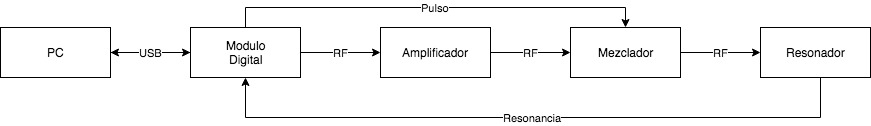
\includegraphics[width=\linewidth]{../figures/d4.jpg}
    \caption{Diagrama de conexiones}
    \label{fig:d4}
\end{figure}
  
%Figure \ref{fig:boat1} shows a boat.

\subsection{Mezclador}

Los pulsos TTL de salida y la se\~nal de radiofrecuencia son las entradas del mezclador
donde se convierten en una sola cuando el pulso TTL est\'a activo en 5 voltios.
Esto permite crear pulsos de estimulaci\'on y relajaci\'on con precisi\'on.

\subsection{Amplificador}
La se\~nal de RF proveniente del \textit{Mezclador} se amplifican tras los efectos de este que debilitan la se\~nal.
La configuraci\'on del mismo var\'ia seg\'un el experimento a realizar.

\subsection{Resonador}
Entre sus partes m\'as relevantes este cuenta con una denominada "malla de acople" la cual
tiene como objetivo dejar pasar la se\~nal RF al contenedor de la muestra e impedir
que contin\'uen a la etapa de adquisici\'on.
La se\~nal de salida de la resonancia es pre-amplificada antes de retornar al \textit{M\'odulo Digital}

\subsection{Configuraci\'on alternativa}
En algunos casos es posible utilizar el \textit{M\'odulo Digital} como generador de pulsos TTL con una fuente
generadora de se\~nal RF externa. Esto no es habitual pero es posible de realizar.

\newpage
